\section{Stereopsis}
Stereopsis, translating literally to ``Solid Appearance'', is the ability to perceive depth. For people with two functioning eyes, this is done sub-consciously by the brain, by observing the differences between the image received by each eye.

Being aware of the depth information in a scene has multiple advantages in the context of this project.

For navigational assistance, it is crucial to be able to know how far away obstacle are, so we are able to warn them that something is blocking their path.

It is also important when conveying the shape or structure of an object to a user. To extract an individual object from an image, we need to know the object boundaries. In a high contrast scenario --- for instance, a red object on a yellow background, this is possible using only image data. However, in a lower-contrast situation, for instance a gray object on a black background, this can be more difficult. This report details a method that allows depth information to be combined with image data, demonstrating improvements over image/depth segmentation alone. 

As traditional cameras are unable to accurately infer depth, a depth-sensing camera must be used to acquire depth information.

In this section of the report, a basic overview of different ways of digitally acquiring depth information is provided.

\subsection{Structured Light}
The Xtion~\cite{xtion} device used in this project uses a technique involving structured light in order to compute the depth-map of a scene.

The Xtion projects a known pattern of structured \ac{IR} laser light onto the scene, and using an \ac{IR} camera, receives the location and shape of each \ac{IR} point. The camera does not use a lens like those found on normal, visible-light cameras --- it has what's known as an astigmatic lens. An astigmatic lens has a focal-length along the X-axis that differs to that along the Y-axis. For instance, if the projected pattern consisted of many circular points, due to astigmatism in the lens, the image read back by the infra-red camera would consist of many elliptical points, varying in eccentricity according to distance between the point and the projector.

Using the change in eccentricity for each point, the device is able to construct a depth-map of the scene in real-time.

\begin{figure}[H]
\centering
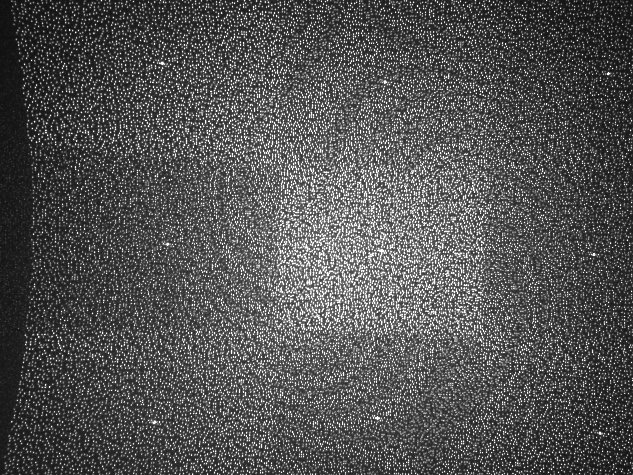
\includegraphics[width=0.6\textwidth]{Theory/kinect_ir_pattern.jpg}
\caption{IR Pattern from Kinect Device~\cite{primesense-irstream}}
\end{figure}

This sensor was developed by a company called Primesense, and is quite well supported --- drivers are available for all major platforms. The Xtion is also supported by OpenNI~\cite{openni}, a framework used to develop software for ``Natural Interaction'' devices. 

\subsection{Other Techniques}
Use of structured light is not the old technique that has been developed to acquire depth-maps - other methods exist, for instance, Time-of-Flight and Stereoscopic systems. The Asus Xtion was chosen over other devices, as it is fairly in-expensive (\~£100), and can be powered by USB alone (other devices, such as the Microsoft Kinect, require mains power to operate). 

\section{Image Segmentation}
There are many different techniques for segmenting images in Computer Vision --- however, there is no ``one size fits all'' solution, each method has pros and cons. 
\label{sec:segment}

This section aims to describe some different methods, along with explanations as to why they are/are not relevant to this project.

\subsection{Histogram Thresholding} 
Histogram Thresholding is a way of segmenting an image into a binary mask consisting of the background and the foreground. This is acheived by analysing the frequency distribution of image intensity values, and choosing a point on this histogram at which to split the image into two parts.  

There are several specific implementations, although they can be generalised into the following form:
\begin{equation}
f: \left\{{0,1,2,...,255}\right\} \rightarrow [0, 1]
\end{equation}

\subsubsection{Example}
Consider this image:

\begin{figure}
    \centering
    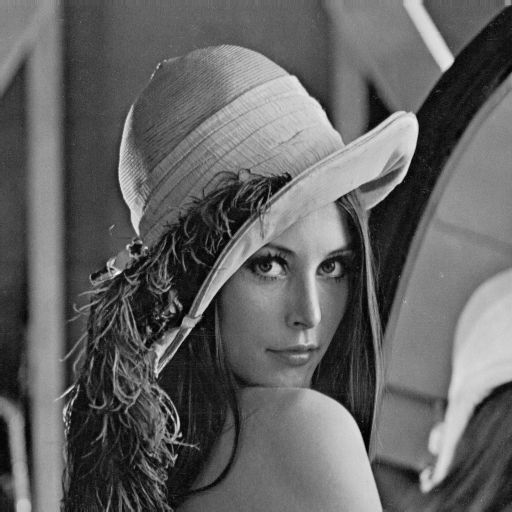
\includegraphics[width=0.33\textwidth]{Theory/lena-grey.jpg}
    \caption{Lena}
\end{figure}

The histogram of this greyscale image is as follows:

\begin{figure}[H]
    \centering
    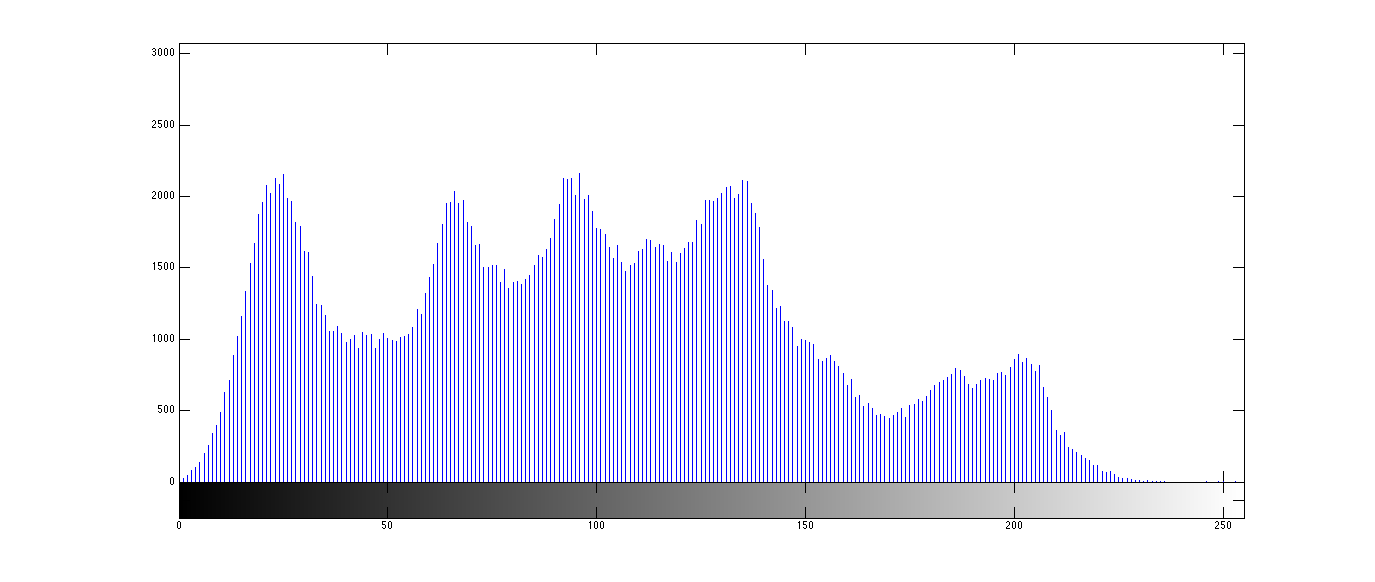
\includegraphics[width=\textwidth]{Theory/lena-grey-hist.png}
    \caption{Histogram of Lena Image}
\end{figure}

The peaks on the histogram correspond to the dominant grey tones in the image --- dark to light, from left to right.

There are various algorithms to choose the exact point on the histogram at which to threshold, each having their own merit. Automatic, un-assisted thresholding is often considered on of the most difficult tasks in Computer Vision (http://www.math.tau.ac.il/~turkel/notes/otsu.pdf), so unless the environment is well-known, alternative methods of segmentation may be more appropriate.

\subsection{Flood Fill}
\label{sec:floodfill}
The flood fill algorithm is used to select an area of an image, based on an initial ``Seed Pixel'' and a threshold value.

A recursive flood-fill algorithm can be described as follows. Neighbouring pixels to the initial seed pixels are examined --- if the difference between the initial seed pixel and the neighbour pixel is less than the given threshold value, then the neighbour pixel is marked as being part of the seed pixel. The algorithm the repeats on all similar neighbouring pixels, always comparing pixels to the \textbf{initial} seed pixel.

\begin{figure}[H]
    \centering
    \begin{subfigure}[b]{0.45\textwidth}
        \centering
        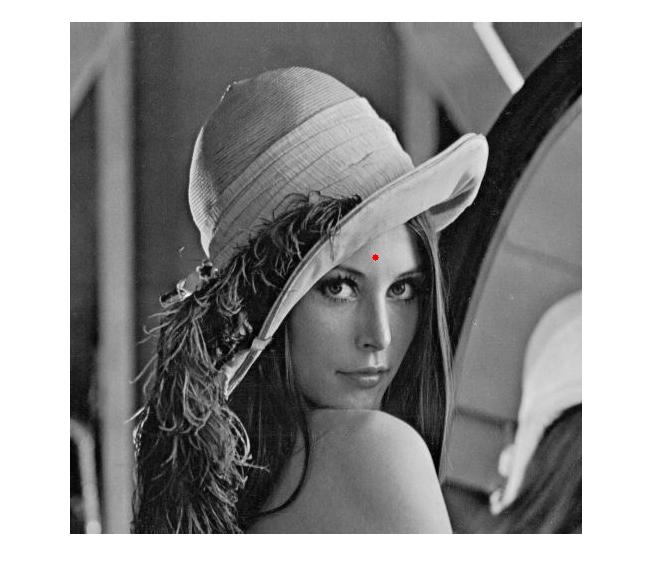
\includegraphics[width=\textwidth]{Theory/lena-dot.png}
        \caption{Initial Seed Point}
    \end{subfigure}
    \begin{subfigure}[b]{0.45\textwidth}
        \centering
        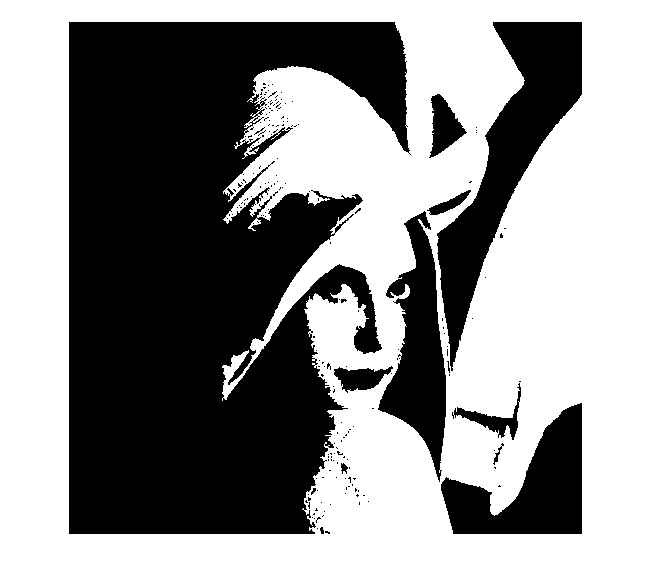
\includegraphics[width=\textwidth]{Theory/lena-dot-thresh.png}
        \caption{After extraction with tolerance=100}
    \end{subfigure}
\end{figure}

This method can work well if the location of the initial seed pixel is known, however, is not so useful if the starting point is unknown.

\subsection{K-Means}
\label{sec:kmeans}
The K-Means algorithm is used to partition a collection of objects into $K$ groups. In the context of Computer Vision, an object is a pixel, and a group is a region.

The algorithm is supplied with $K$ initial colours - ideally (but not necessarily) belonging to the $K$ regions that the image should be segmented into. These colours are known as ``Initial Group Centroids''.

Each pixel in the image is assigned to the most similar centroid. The value of the centroid is then updated to be set to the mean of it's member pixels.

This process is then repeated, with the value of the centroid being updated with each pass - this can be done a fixed number of times, or until each centroid value converges.

\subsubsection{Example}
The following is an example of the result of K-means clustering with $K = 3$, with randomly selected Initial Group Centroids.

\begin{figure}[H]
    \centering
    \begin{subfigure}[b]{0.45\textwidth}
        \centering
        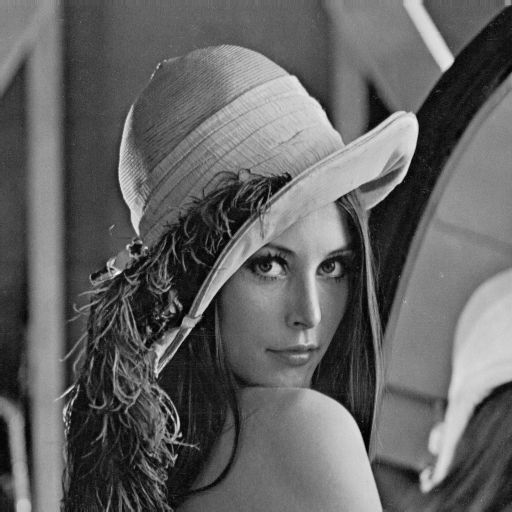
\includegraphics[width=\textwidth]{Theory/lena-grey.jpg}
        \caption{Input Image}
    \end{subfigure}
    \begin{subfigure}[b]{0.45\textwidth}
        \centering
        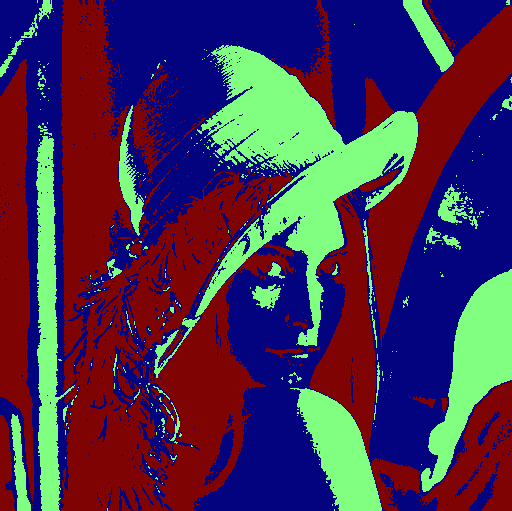
\includegraphics[width=\textwidth]{Theory/lena-kmeans.png}
        \caption{K-Means clustering, with $K = 3$}
    \end{subfigure}
\end{figure}

\section{Elliptic Fourier Descriptors}
Elliptic Fourier Descriptors are the result of performing an \ac{EFT}, and can be used to describe the shape of a contour.

Before computing the EFD of an image, its contour needs to be extracted. This can be be done by segmenting the image (using a technique described in \ref{sec:segment}), then finding the outermost contour of the segment. This can be done using one of many possible contour tracing techniques, such as Moore Neighbourhood Tracing.

\subsection{Chain Code}
The first step of the Elliptic Fourier Transform is to compute the chain code of the contour.

Chain codes are used to losslesly encode a monochrome image --- they describe the connectivity of a list of points, relative to each point.

\section{Image Moments}
Formally, the moment of an image can be defined as\cite{liao1996image}:

\begin{equation}
M_{ij} = \sum_x \sum_y x^i y^j I(x,y)\,\!
\end{equation}

That is, the sum of pixel intensities, waited according to the $x$ and $y$ co-ordinates of each pixel co-ordinate raised to parameters $i$ and $j$ respectively.

Certain properties of images can be established by using particular $i$ and $j$ values during moment calculation - for instance for a Binary Image, area can be given by: $M_{00}$, and image centroid can be given by ${x, y} = M_{10}/M_{00}, M_{01}/M_{00}$.


\subsection{Hu Invariant Moments}
\label{sec:hu}
Hu's Invariant Moments~\cite{hu1962visual} are a set of 7 image moments:

$I_1 = \eta_{20} + \eta_{02}$

$I_2 = (\eta_{20} - \eta_{02})^2 + 4\eta_{11}^2$

$I_3 = (\eta_{30} - 3\eta_{12})^2 + (3\eta_{21} - \eta_{03})^2$

$I_4 = (\eta_{30} + \eta_{12})^2 + (\eta_{21} + \eta_{03})^2$

$I_5 = (\eta_{30} - 3\eta_{12}) (\eta_{30} + \eta_{12})[ (\eta_{30} + \eta_{12})^2 - 3 (\eta_{21} + \eta_{03})^2] + (3 \eta_{21} - \eta_{03}) (\eta_{21} + \eta_{03})[ 3(\eta_{30} + \eta_{12})^2 -  (\eta_{21} + \eta_{03})^2]$

$I_6 =  (\eta_{20} - \eta_{02})[(\eta_{30} + \eta_{12})^2 - (\eta_{21} + \eta_{03})^2] + 4\eta_{11}(\eta_{30} + \eta_{12})(\eta_{21} + \eta_{03})$

$I_7 = (3 \eta_{21} - \eta_{03})(\eta_{30} + \eta_{12})[(\eta_{30} + \eta_{12})^2 - 3(\eta_{21} + \eta_{03})^2] - (\eta_{30} - 3\eta_{12})(\eta_{21} + \eta_{03})[3(\eta_{30} + \eta_{12})^2 - (\eta_{21} + \eta_{03})^2]$

where $\eta_{ij}$ is the scale-invariant moment given by:

$\eta_{ij} = \frac{\mu_{ij}} {\mu_{00}^{\left(1 + \frac{i+j}{2}\right)}}\,\!$

and $\mu_{ij}$ is the central moment, given by:

$\mu_{ij} = \sum_{x} \sum_{y} (x - \bar{x})^i(y - \bar{y})^j f(x,y)$

As the name name suggests, values resulting from calculating $I_{1..7}$ are invariant to scale, rotation and translation --- that is, they remain constant no matter their size, their location or angle they are at. 

\subsection{Zernike Moment Descriptors}
\label{sec:zernike}
Zernike Moments are not dissimilar to normal image moments, however are calculated differently --- they are based on Complex Zernike Polynomials~\cite{liao1997image}.

Zernike Moments are orthogonal --- that is, each Zernike moment is statically independent from another, meaning there is little redundancy~\cite{amayeh2005accurate}. This means that using Zernike Moments is an efficient way of parameterizing an image.
